% Copyright 2004 by Till Tantau <tantau@users.sourceforge.net>.
%
% In principle, this file can be redistributed and/or modified under
% the terms of the GNU Public License, version 2.
%
% However, this file is supposed to be a template to be modified
% for your own needs. For this reason, if you use this file as a
% template and not specifically distribute it as part of a another
% package/program, I grant the extra permission to freely copy and
% modify this file as you see fit and even to delete this copyright
% notice.
\documentclass[aspectratio=169,table]{beamer}
\usepackage[T1]{fontenc}
\usepackage[utf8]{inputenc}
\usepackage{graphicx}
\usepackage[brazil,english]{babel}
\usepackage[alf,abnt-etal-cite=2]{abntex2cite}
\usepackage{lipsum}
\usepackage{tikz}
\usepackage{amsmath}


\usetikzlibrary{arrows,shapes}


% There are many different themes available for Beamer. A comprehensive
% list with examples is given here:
% http://deic.uab.es/~iblanes/beamer_gallery/index_by_theme.html
% You can uncomment the themes below if you would like to use a different
% one:
%\usetheme{AnnArbor}
%\usetheme{Antibes}
%\usetheme{Bergen}
%\usetheme{Berkeley}
%\usetheme{Berlin}
%\usetheme{Boadilla}
%\usetheme{boxes}
%\usetheme{CambridgeUS}
%\usetheme{Copenhagen}
%\usetheme{Darmstadt}
%\usetheme{Dresden}
%\usetheme{default}
\usetheme{Frankfurt}
%\usetheme{Goettingen}
%\usetheme{Hannover}
%\usetheme{Ilmenau}
%\usetheme{JuanLesPins}
%\usetheme{Luebeck}
%\usetheme{Madrid}
%\usetheme{Malmoe}
%\usetheme{Marburg}
%\usetheme{Montpellier}
%\usetheme{PaloAlto}
%\usetheme{Pittsburgh}
%\usetheme{Rochester}
%\usetheme{Singapore}
%\usetheme{Szeged}
%\usetheme{Warsaw}
%\usecolortheme{orchid}

%%% CUSTON THEME CHAMALEON %%%
\definecolor{chameleongreen1}{RGB}{98,189,25}
\definecolor{chameleongreen2}{RGB}{188,225,141}
\definecolor{chameleongreen3}{RGB}{51,149,48}
\definecolor{chameleongreen4}{RGB}{0,98,90}

\setbeamercolor*{palette primary}{fg=white,bg=chameleongreen1}
\setbeamercolor*{palette secondary}{fg=white,bg=chameleongreen3}
\setbeamercolor*{palette tertiary}{fg=white,bg=chameleongreen4}
\setbeamercolor*{palette quaternary}{fg=white,bg=chameleongreen4}

\setbeamercolor*{titlelike}{bg=chameleongreen3}
%edited
\setbeamercolor*{frametitle}{bg=chameleongreen3,fg=white}
%
\setbeamercolor*{part title}{bg=black,fg=black}
\setbeamercolor*{item}{fg=chameleongreen3}

\setbeamercolor*{separation line}{}
\setbeamercolor*{fine separation line}{}

%%% END CUSTOM THEME %%%


%\setbeamercolor{frametitle}{bg=white,fg=black}
\setbeamercolor{page number in head/foot}{bg=chameleongreen3,fg=chameleongreen2}
\setbeamerfont{frametitle}{series=\bfseries}
\setbeamertemplate{navigation symbols}{}

\setbeamertemplate{footline}
{%
  \leavevmode%
  \hbox{\begin{beamercolorbox}[wd=.5\paperwidth,ht=2.5ex,dp=1.125ex,leftskip=.3cm plus1fill,rightskip=.3cm]{author in head/foot}%
	\usebeamerfont{author in head/foot}\insertshortauthor
  \end{beamercolorbox}%
  \begin{beamercolorbox}[wd=.45\paperwidth,ht=2.5ex,dp=1.125ex,leftskip=.3cm,rightskip=.3cm plus1fil]{title in head/foot}%
	\usebeamerfont{title in head/foot}\insertshortinstitute
  \end{beamercolorbox}%
  \begin{beamercolorbox}[wd=.05\paperwidth,ht=2.5ex,dp=1.125ex,leftskip=.1cm,rightskip=.1cm plus1fil]{page number in head/foot}
  \center\usebeamerfont{page number in head/foot}\insertframenumber
  \end{beamercolorbox}}%
  \vskip0pt%
}

%\title{Um modelo do contexto de busca do usuário para personalização de resultados na Web}
\title{Métodos de Ordenação}

% A subtitle is optional and this may be deleted
\subtitle{Comb Sort}

\author[Orsoletta{,} B. D.; Weber{,} D. R.; Debastiani{,} T. A.]{Bruno Dall Orsoleta, Dayan Roberto Weber, Tiago Adalberto Debastiani}
% - Give the names in the same order as the appear in the paper.
% - Use the \inst{?} command only if the authors have different
%   affiliation.

\institute[UFFS -- \textit{Campus} Chapecó] % (optional, but mostly needed)
{%
  Estrutura de Dados I\\%
  Ciência da Computação\\%
  Universidade Federal da Fronteira Sul\\%
  \textit{Campus} Chapecó%
}
% - Use the \inst command only if there are several affiliations.
% - Keep it simple, no one is interested in your street address.

\date{Junho, 2016}
% - Either use conference name or its abbreviation.
% - Not really informative to the audience, more for people (including
%   yourself) who are reading the slides online

%\subject{Theoretical Computer Science}
% This is only inserted into the PDF information catalog. Can be left
% out.

% If you have a file called "university-logo-filename.xxx", where xxx
% is a graphic format that can be processed by latex or pdflatex,
% resp., then you can add a logo as follows:
% 
\includegraphics[height=1cm]{marca_uffs.eps}
 \pgfdeclareimage[height=1cm]{university-logo}{marca_uffs}
 \logo{\pgfuseimage{university-logo}}

% Delete this, if you do not want the table of contents to pop up at
% the beginning of each subsection:
% \AtBeginSubsection[]
% {
%   \begin{frame}<beamer>{Agenda}
%     \tableofcontents[currentsection,currentsubsection]
%   \end{frame}
% }

\AtBeginSection[]
{
  \begin{frame}<beamer>{Agenda}
	\tableofcontents[currentsection]
  \end{frame}
}

% Let's get started
\begin{document}
% For every picture that defines or uses external nodes, you'll have to
% apply the 'remember picture' style. To avoid some typing, we'll apply
% the style to all pictures.
\tikzstyle{every picture}+=[remember picture]

% By default all math in TikZ nodes are set in inline mode. Change this to
% displaystyle so that we don't get small fractions.
\everymath{\displaystyle}


\begin{frame}[label=titlepage]
  \titlepage
\end{frame}

% \begin{frame}{Agenda}
%   \tableofcontents
%   % You might wish to add the option [pausesections]
% \end{frame}

% Section and subsections will appear in the presentation overview
% and table of contents.
%\section{Problemática}
\section{Sobre}
	\subsection{Como Surgiu?}
		\begin{frame}
			\frametitle{\secname}
			\framesubtitle{\subsecname}
			\begin{itemize}
				\item Desenvolvido em 1980 por Wlodzimierz Dobosiewicz. Redescoberto e popularizado por Stephen Lacey e Richard Box em um artigo publicado na revista Byte em Abril de 1991;
				\item Compara diferentes itens separados por um salto, semelhante ao \textbf{Bubble Sort}, porém, o \textit{gap} (Distância entre os itens) no Comb Sort é definido por um \textbf{fator de encolhimento};
				\item O \textit{gap} inicia com o comprimento da lista dividido pelo fator de encolhimento, e a cada iteração seu valor é dividido novamente por esse fator, até seu valor ser igual a 1;
			\end{itemize}
		\end{frame}
	\subsection{Fator de Encolhimento}
		\begin{frame}
			\frametitle{\secname}
			\framesubtitle{\subsecname}
			\begin{itemize}
				\item O fator foi definido após testar o algoritmo em mais de 200\,000 listas aleatórias, com cerca de 1\,000 a 1\,040 elementos, com o fator de encolhimento variando de 1.1 a 1.5;
				\item ``[\dots] o Fator de Encolhimento (FE) ótimo é próximo a 1.3. FE = 1.15 é lento pelo excesso de comparações; FE = 1.45 é erraticamente lento pois pouquíssimos \textit{turtles} são resolvidos. Disso e de pontos semelhantes, nos ficou claro que 1.3 é o melhor casamento de consistência e velocidade.''\cite{comb1991}
			\end{itemize}
			\begin{figure}
				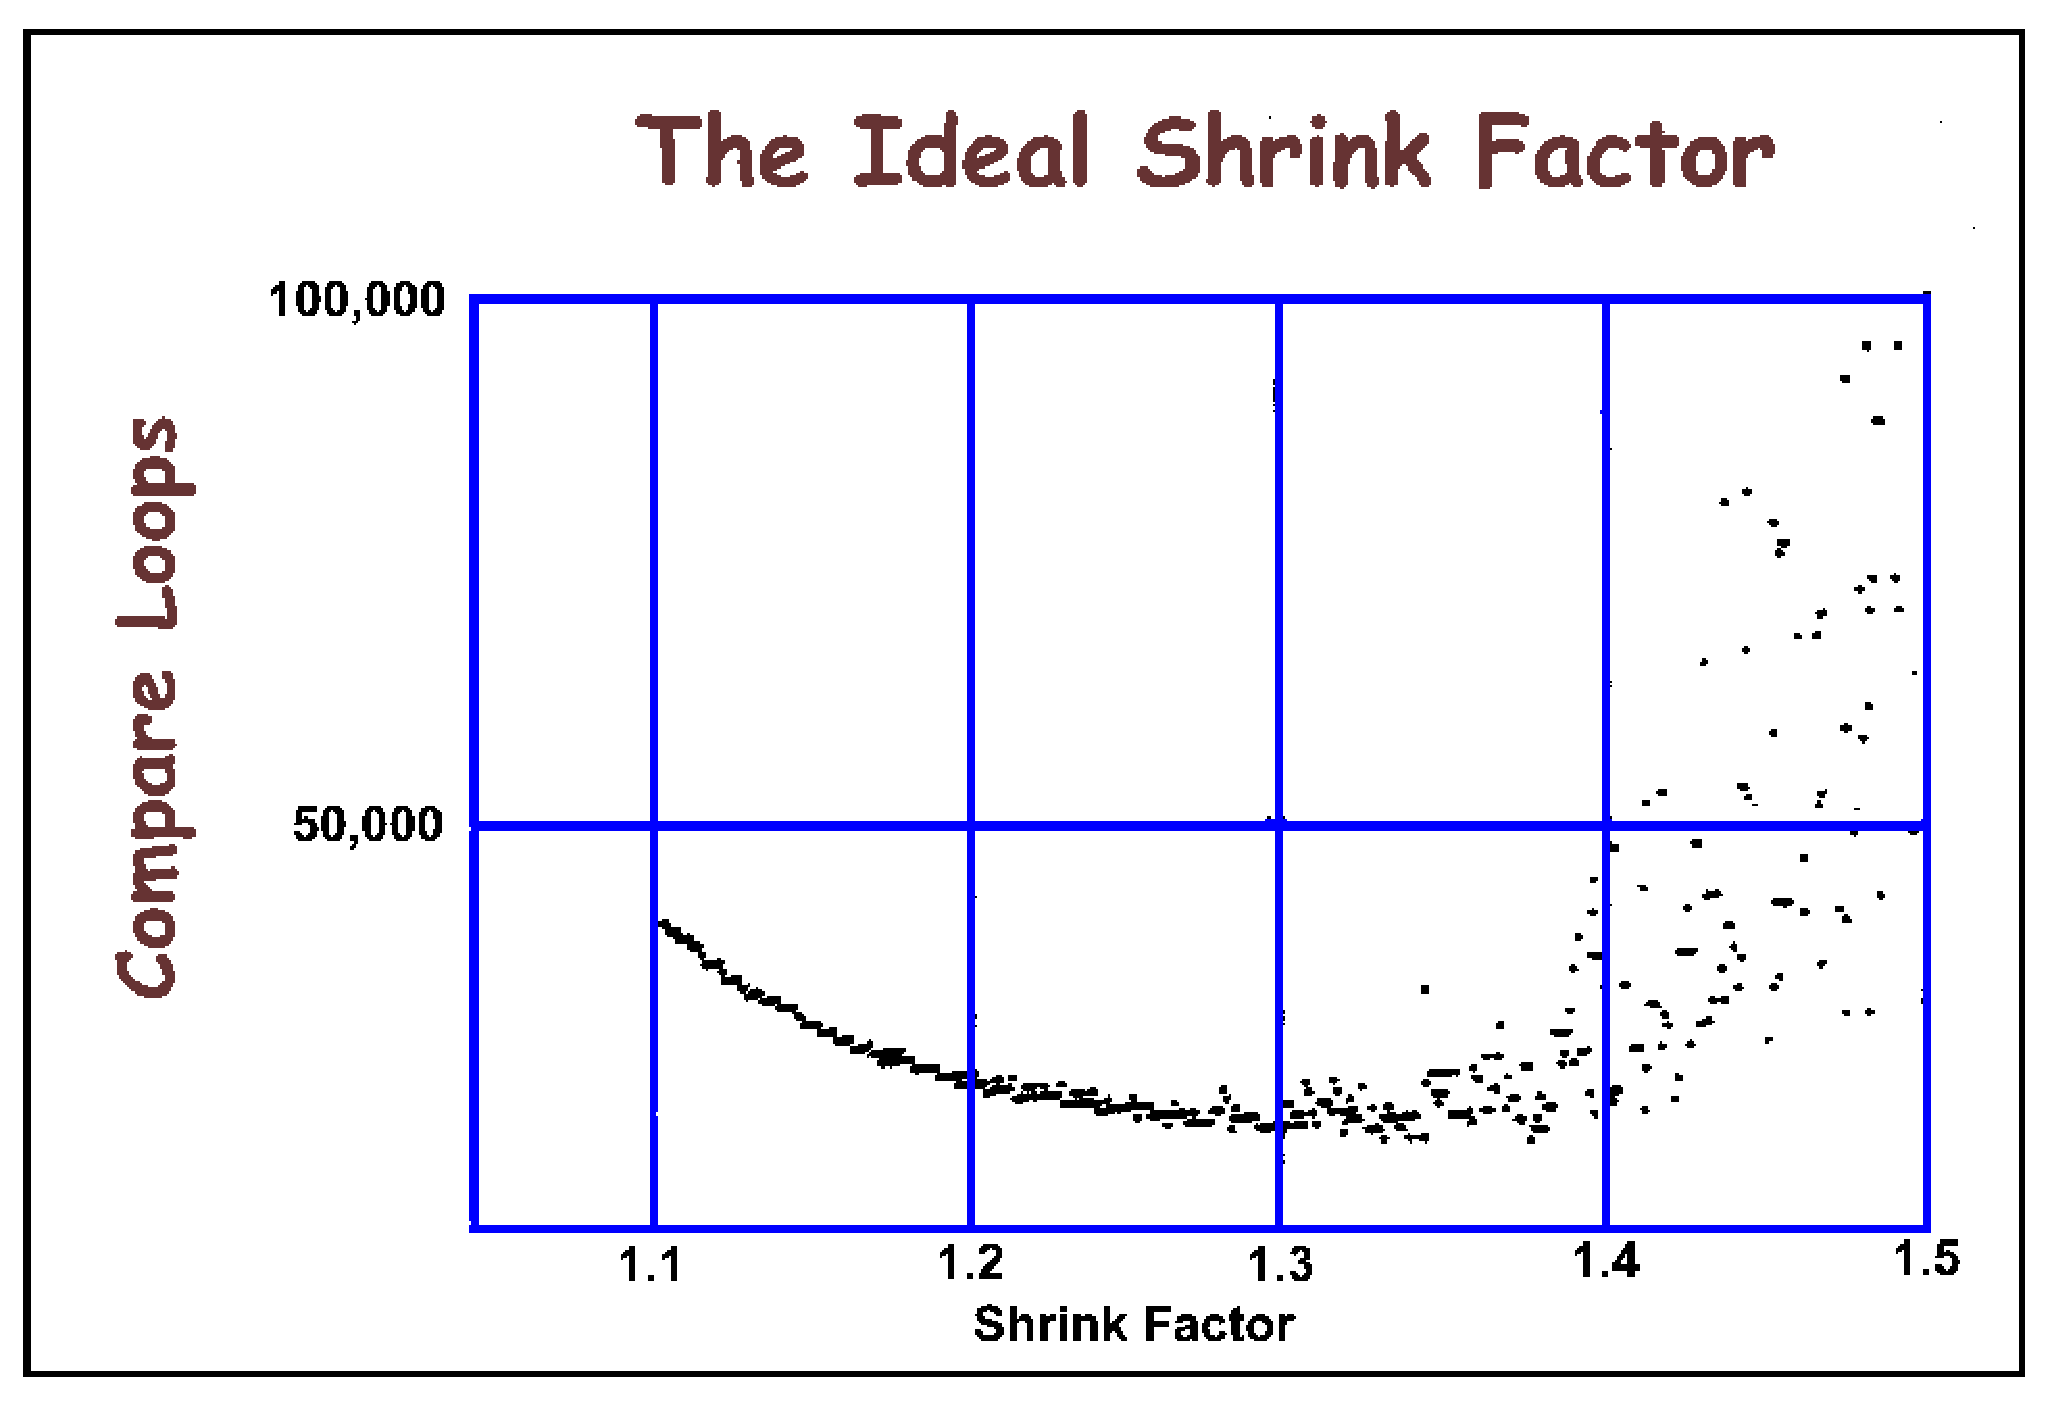
\includegraphics[height=.3\textheight]{Imagens/gap_image}
				\label{fig:perguntas}
			\end{figure}
		\end{frame}

\section{Como funciona?}
	\subsection{Exempo prático}
		\begin{frame}
		\frametitle{\secname}
		\framesubtitle{\subsecname}
				
			\begin{description}
				\item[gap] = tam/FE = $^{10}/_{1.3}$ = 7;
				\item[swap] = false;
				\item[i] = 0; \tikz\node[coordinate] (n2) {};
				\item[j] = i + gap = 7; \tikz\node[coordinate] (n1) {};
			\end{description}

			\begin{table}[!htb]
				\centering
					\begin{tabular}{|l|c|c|c|c|c|c|c|c|c|c|}
						\hline
						\rowcolor{chameleongreen3}Posição     & \tikz\node(t2){0}; & 1 & 2 & 3 & 4 & 5 & 6 & \tikz\node(t1){7}; & 8 & 9\\ \hline
						\rowcolor{chameleongreen2}\cellcolor{chameleongreen3}Valor       & \tikz\node(n3){2}; & 4 & 9 & 0 & 1 & 7 & 5 & \tikz\node(t3){3}; & 8 & 6\\ \hline
					\end{tabular}
			\end{table}
			\begin{tikzpicture}[overlay]
				\path[->] (n1) edge [out=0, in=90] (t1);
				\path[->] (n2) edge [out=0, in=90] (t2);
				\path[->] (n3) edge [out=-90, in=-90] node[below] {\footnotesize{menor}} (t3);
			\end{tikzpicture}
		\end{frame}

		\begin{frame}
		\frametitle{\secname}
		\framesubtitle{\subsecname}
				
			\begin{description}
				\item[gap] = 7;
				\item[swap] = false;
				\item[i] = 1; \tikz\node[coordinate] (n2) {};
				\item[j] = i + gap = 8; \tikz\node[coordinate] (n1) {};
			\end{description}

			\begin{table}[!htb]
				\centering
					\begin{tabular}{|l|c|c|c|c|c|c|c|c|c|c|}
						\hline
						\rowcolor{chameleongreen3}Posição     & 0 & \tikz\node(t2){1}; & 2 & 3 & 4 & 5 & 6 & 7 & \tikz\node(t1){8}; & 9\\ \hline
						\rowcolor{chameleongreen2}\cellcolor{chameleongreen3}Valor       & 2 & \tikz\node(n3){4}; & 9 & 0 & 1 & 7 & 5 & 3 & \tikz\node(t3){8}; & 6\\ \hline
					\end{tabular}
			\end{table}
			\begin{tikzpicture}[overlay]
				\path[->] (n1) edge [out=0, in=90] (t1);
				\path[->] (n2) edge [out=0, in=90] (t2);
				\path[->] (n3) edge [out=-90, in=-90] node[below] {\footnotesize{menor}} (t3);
			\end{tikzpicture}
		\end{frame}
	
		\begin{frame}
		\frametitle{\secname}
		\framesubtitle{\subsecname}
				
			\begin{description}
				\item[gap] = 7;
				\item[swap] = false; 
				\item[i] = 2; \tikz\node[coordinate] (n2) {};
				\item[j] = i + gap = 9; \tikz\node[coordinate] (n1) {};
			\end{description}

			\begin{table}[!htb]
				\centering
					\begin{tabular}{|l|c|c|c|c|c|c|c|c|c|c|}
						\hline
						\rowcolor{chameleongreen3}Posição     & 0 & 1 & \tikz\node(t2){2}; & 3 & 4 & 5 & 6 & 7 & 8 & \tikz\node(t1){9};\\ \hline
						\rowcolor{chameleongreen2}\cellcolor{chameleongreen3}Valor       & 2 & 4 & \tikz\node(n3){9}; & 0 & 1 & 7 & 5 & 3 & 8 & \tikz\node(t3){6};\\ \hline
					\end{tabular}
			\end{table}
			\begin{tikzpicture}[overlay]
				\path[->] (n1) edge [out=0, in=90] (t1);
				\path[->] (n2) edge [out=0, in=90] (t2);
				\path[<->,red] (n3) edge [out=-90, in=-90] node[below] {\footnotesize{troca}} (t3);
			\end{tikzpicture}
		\end{frame}

		\begin{frame}
		\frametitle{\secname}
		\framesubtitle{\subsecname}
				
			\begin{description}
				\item[gap] = 7;
				\item[swap] = true; 
				\item[i] = 2; \tikz\node[coordinate] (n2) {};
				\item[j] = i + gap = 9; \tikz\node[coordinate] (n1) {};
			\end{description}

			\begin{table}[!htb]
				\centering
					\begin{tabular}{|l|c|c|c|c|c|c|c|c|c|c|}
						\hline
						\rowcolor{chameleongreen3}Posição     & 0 & 1 & \tikz\node(t2){2}; & 3 & 4 & 5 & 6 & 7 & 8 & \tikz\node(t1){9};\\ \hline
						\rowcolor{chameleongreen2}\cellcolor{chameleongreen3}Valor       & 2 & 4 & \tikz\node(n3){6}; & 0 & 1 & 7 & 5 & 3 & 8 & \tikz\node(t3){9};\\ \hline
					\end{tabular}
			\end{table}
			\begin{tikzpicture}[overlay]
				\path[->] (n1) edge [out=0, in=90] (t1);
				\path[->] (n2) edge [out=0, in=90] (t2);
				\path[<->,red] (n3) edge [out=-90, in=-90] node[below] {\footnotesize{troca}} (t3);
			\end{tikzpicture}
		\end{frame}

		\begin{frame}
		\frametitle{\secname}
		\framesubtitle{\subsecname}
				
			\begin{description}
				\item[gap] = gap/FE = $^7/_{1.3}$ = 5;
				\item[swap] = false;
				\item[i] = 0; \tikz\node[coordinate] (n2) {};
				\item[j] = i + gap = 5; \tikz\node[coordinate] (n1) {};
			\end{description}

			\begin{table}[!htb]
				\centering
					\begin{tabular}{|l|c|c|c|c|c|c|c|c|c|c|}
						\hline
						\rowcolor{chameleongreen3}Posição     & \tikz\node(t2){0}; & 1 & 2 & 3 & 4 & \tikz\node(t1){5}; & 6 & 7 & 8 & 9\\ \hline
						\rowcolor{chameleongreen2}\cellcolor{chameleongreen3}Valor       & \tikz\node(n3){2}; & 4 & 6 & 0 & 1 & \tikz\node(t3){7}; & 5 & 3 & 8 & 9\\ \hline
					\end{tabular}
			\end{table}
			\begin{tikzpicture}[overlay]
				\path[->] (n1) edge [out=0, in=90] (t1);
				\path[->] (n2) edge [out=0, in=90] (t2);
				\path[->] (n3) edge [out=-90, in=-90] node[below] {\footnotesize{menor}} (t3);
			\end{tikzpicture}
		\end{frame}

		\begin{frame}
		\frametitle{\secname}
		\framesubtitle{\subsecname}
				
			\begin{description}
				\item[gap] = 5;
				\item[swap] = false;
				\item[i] = 1; \tikz\node[coordinate] (n2) {};
				\item[j] = i + gap = 6; \tikz\node[coordinate] (n1) {};
			\end{description}

			\begin{table}[!htb]
				\centering
					\begin{tabular}{|l|c|c|c|c|c|c|c|c|c|c|}
						\hline
						\rowcolor{chameleongreen3}Posição     & 0 & \tikz\node(t2){1}; & 2 & 3 & 4 & 5 & \tikz\node(t1){6}; & 7 & 8 & 9\\ \hline
						\rowcolor{chameleongreen2}\cellcolor{chameleongreen3}Valor       & 2 & \tikz\node(n3){4}; & 6 & 0 & 1 & 7 & \tikz\node(t3){5}; & 3 & 8 & 9\\ \hline
					\end{tabular}
			\end{table}
			\begin{tikzpicture}[overlay]
				\path[->] (n1) edge [out=0, in=90] (t1);
				\path[->] (n2) edge [out=0, in=90] (t2);
				\path[->] (n3) edge [out=-90, in=-90] node[below] {\footnotesize{menor}} (t3);
			\end{tikzpicture}
		\end{frame}

		\begin{frame}
		\frametitle{\secname}
		\framesubtitle{\subsecname}
				
			\begin{description}
				\item[gap] = 5; 
				\item[swap] = false;
				\item[i] = 2; \tikz\node[coordinate] (n2) {};
				\item[j] = i + gap = 7; \tikz\node[coordinate] (n1) {};
			\end{description}

			\begin{table}[!htb]
				\centering
					\begin{tabular}{|l|c|c|c|c|c|c|c|c|c|c|}
						\hline
						\rowcolor{chameleongreen3}Posição     & 0 & 1 & \tikz\node(t2){2}; & 3 & 4 & 5 & 6 & \tikz\node(t1){7}; & 8 & 9\\ \hline
						\rowcolor{chameleongreen2}\cellcolor{chameleongreen3}Valor       & 2 & 4 & \tikz\node(n3){6}; & 0 & 1 & 7 & 5 & \tikz\node(t3){3}; & 8 & 9\\ \hline
					\end{tabular}
			\end{table}
			\begin{tikzpicture}[overlay]
				\path[->] (n1) edge [out=0, in=90] (t1);
				\path[->] (n2) edge [out=0, in=90] (t2);
				\path[<->,red] (n3) edge [out=-90, in=-90] node[below] {\footnotesize{troca}} (t3);
			\end{tikzpicture}
		\end{frame}

		\begin{frame}
		\frametitle{\secname}
		\framesubtitle{\subsecname}
				
			\begin{description}
				\item[gap] = 5; 
				\item[swap] = true;
				\item[i] = 2; \tikz\node[coordinate] (n2) {};
				\item[j] = i + gap = 7; \tikz\node[coordinate] (n1) {};
			\end{description}

			\begin{table}[!htb]
				\centering
					\begin{tabular}{|l|c|c|c|c|c|c|c|c|c|c|}
						\hline
						\rowcolor{chameleongreen3}Posição     & 0 & 1 & \tikz\node(t2){2}; & 3 & 4 & 5 & 6 & \tikz\node(t1){7}; & 8 & 9\\ \hline
						\rowcolor{chameleongreen2}\cellcolor{chameleongreen3}Valor       & 2 & 4 & \tikz\node(n3){3}; & 0 & 1 & 7 & 5 & \tikz\node(t3){6}; & 8 & 9\\ \hline
					\end{tabular}
			\end{table}
			\begin{tikzpicture}[overlay]
				\path[->] (n1) edge [out=0, in=90] (t1);
				\path[->] (n2) edge [out=0, in=90] (t2);
				\path[<->,red] (n3) edge [out=-90, in=-90] node[below] {\footnotesize{troca}} (t3);
			\end{tikzpicture}
		\end{frame}

		\begin{frame}
		\frametitle{\secname}
		\framesubtitle{\subsecname}
				
			\begin{description}
				\item[gap] = 5;
				\item[swap] = true;
				\item[i] = 3; \tikz\node[coordinate] (n2) {};
				\item[j] = i + gap = 8; \tikz\node[coordinate] (n1) {};
			\end{description}

			\begin{table}[!htb]
				\centering
					\begin{tabular}{|l|c|c|c|c|c|c|c|c|c|c|}
						\hline
						\rowcolor{chameleongreen3}Posição     & 0 & 1 & 2 & \tikz\node(t2){3}; & 4 & 5 & 6 & 7 & \tikz\node(t1){8}; & 9\\ \hline
						\rowcolor{chameleongreen2}\cellcolor{chameleongreen3}Valor       & 2 & 4 & 3 & \tikz\node(n3){0}; & 1 & 7 & 5 & 6 & \tikz\node(t3){8}; & 9\\ \hline
					\end{tabular}
			\end{table}
			\begin{tikzpicture}[overlay]
				\path[->] (n1) edge [out=0, in=90] (t1);
				\path[->] (n2) edge [out=0, in=90] (t2);
				\path[->] (n3) edge [out=-90, in=-90] node[below] {\footnotesize{menor}} (t3);
			\end{tikzpicture}
		\end{frame}

		\begin{frame}
		\frametitle{\secname}
		\framesubtitle{\subsecname}
				
			\begin{description}
				\item[gap] = 5;
				\item[swap] = true;
				\item[i] = 4; \tikz\node[coordinate] (n2) {};
				\item[j] = i + gap = 9; \tikz\node[coordinate] (n1) {};
			\end{description}

			\begin{table}[!htb]
				\centering
					\begin{tabular}{|l|c|c|c|c|c|c|c|c|c|c|}
						\hline
						\rowcolor{chameleongreen3}Posição     & 0 & 1 & 2 & 3 & \tikz\node(t2){4}; & 5 & 6 & 7 & 8 & \tikz\node(t1){9};\\ \hline
						\rowcolor{chameleongreen2}\cellcolor{chameleongreen3}Valor       & 2 & 4 & 3 & 0 & \tikz\node(n3){1}; & 7 & 5 & 6 & 8 & \tikz\node(t3){9};\\ \hline
					\end{tabular}
			\end{table}
			\begin{tikzpicture}[overlay]
				\path[->] (n1) edge [out=0, in=90] (t1);
				\path[->] (n2) edge [out=0, in=90] (t2);
				\path[->] (n3) edge [out=-90, in=-90] node[below] {\footnotesize{menor}} (t3);
			\end{tikzpicture}
		\end{frame}

		\begin{frame}
		\frametitle{\secname}
		\framesubtitle{\subsecname}
				
			\begin{description}
				\item[gap] = gap/FE = $^5/_{1.3}$ = 3;
				\item[swap] = false;
				\item[i] = 0; \tikz\node[coordinate] (n2) {};
				\item[j] = i + gap = 3; \tikz\node[coordinate] (n1) {};
			\end{description}

			\begin{table}[!htb]
				\centering
					\begin{tabular}{|l|c|c|c|c|c|c|c|c|c|c|}
						\hline
						\rowcolor{chameleongreen3}Posição     & \tikz\node(t2){0}; & 1 & 2 & \tikz\node(t1){3}; & 4 & 5 & 6 & 7 & 8 & 9\\ \hline
						\rowcolor{chameleongreen2}\cellcolor{chameleongreen3}Valor       & \tikz\node(n3){2}; & 4 & 3 & \tikz\node(t3){0}; & 1 & 7 & 5 & 6 & 8 & 9\\ \hline
					\end{tabular}
			\end{table}
			\begin{tikzpicture}[overlay]
				\path[->] (n1) edge [out=0, in=90] (t1);
				\path[->] (n2) edge [out=0, in=90] (t2);
				\path[<->,red] (n3) edge [out=-90, in=-90] node[below] {\footnotesize{troca}} (t3);
			\end{tikzpicture}
		\end{frame}

		\begin{frame}
		\frametitle{\secname}
		\framesubtitle{\subsecname}
				
			\begin{description}
				\item[gap] = 3;
				\item[swap] = true;
				\item[i] = 0; \tikz\node[coordinate] (n2) {};
				\item[j] = i + gap = 3; \tikz\node[coordinate] (n1) {};
			\end{description}

			\begin{table}[!htb]
				\centering
					\begin{tabular}{|l|c|c|c|c|c|c|c|c|c|c|}
						\hline
						\rowcolor{chameleongreen3}Posição     & \tikz\node(t2){0}; & 1 & 2 & \tikz\node(t1){3}; & 4 & 5 & 6 & 7 & 8 & 9\\ \hline
						\rowcolor{chameleongreen2}\cellcolor{chameleongreen3}Valor       & \tikz\node(n3){0}; & 4 & 3 & \tikz\node(t3){2}; & 1 & 7 & 5 & 6 & 8 & 9\\ \hline
					\end{tabular}
			\end{table}
			\begin{tikzpicture}[overlay]
				\path[->] (n1) edge [out=0, in=90] (t1);
				\path[->] (n2) edge [out=0, in=90] (t2);
				\path[<->,red] (n3) edge [out=-90, in=-90] node[below] {\footnotesize{troca}} (t3);
			\end{tikzpicture}
		\end{frame}

		\begin{frame}
		\frametitle{\secname}
		\framesubtitle{\subsecname}
				
			\begin{description}
				\item[gap] = 3;
				\item[swap] = true; 
				\item[i] = 1; \tikz\node[coordinate] (n2) {};
				\item[j] = i + gap = 4; \tikz\node[coordinate] (n1) {};
			\end{description}

			\begin{table}[!htb]
				\centering
					\begin{tabular}{|l|c|c|c|c|c|c|c|c|c|c|}
						\hline
						\rowcolor{chameleongreen3}Posição     & 0 & \tikz\node(t2){1}; & 2 & 3 & \tikz\node(t1){4}; & 5 & 6 & 7 & 8 & 9\\ \hline
						\rowcolor{chameleongreen2}\cellcolor{chameleongreen3}Valor       & 0 & \tikz\node(n3){4}; & 3 & 2 & \tikz\node(t3){1}; & 7 & 5 & 6 & 8 & 9\\ \hline
					\end{tabular}
			\end{table}
			\begin{tikzpicture}[overlay]
				\path[->] (n1) edge [out=0, in=90] (t1);
				\path[->] (n2) edge [out=0, in=90] (t2);
				\path[<->,red] (n3) edge [out=-90, in=-90] node[below] {\footnotesize{troca}} (t3);
			\end{tikzpicture}
		\end{frame}

		\begin{frame}
		\frametitle{\secname}
		\framesubtitle{\subsecname}
				
			\begin{description}
				\item[gap] = 3;
				\item[swap] = true; 
				\item[i] = 1; \tikz\node[coordinate] (n2) {};
				\item[j] = i + gap = 4; \tikz\node[coordinate] (n1) {};
			\end{description}

			\begin{table}[!htb]
				\centering
					\begin{tabular}{|l|c|c|c|c|c|c|c|c|c|c|}
						\hline
						\rowcolor{chameleongreen3}Posição     & 0 & \tikz\node(t2){1}; & 2 & 3 & \tikz\node(t1){4}; & 5 & 6 & 7 & 8 & 9\\ \hline
						\rowcolor{chameleongreen2}\cellcolor{chameleongreen3}Valor       & 0 & \tikz\node(n3){1}; & 3 & 2 & \tikz\node(t3){4}; & 7 & 5 & 6 & 8 & 9\\ \hline
					\end{tabular}
			\end{table}
			\begin{tikzpicture}[overlay]
				\path[->] (n1) edge [out=0, in=90] (t1);
				\path[->] (n2) edge [out=0, in=90] (t2);
				\path[<->,red] (n3) edge [out=-90, in=-90] node[below] {\footnotesize{troca}} (t3);
			\end{tikzpicture}
		\end{frame}

		\begin{frame}
		\frametitle{\secname}
		\framesubtitle{\subsecname}
				
			\begin{description}
				\item[gap] = 3;
				\item[swap] = true;
				\item[i] = 2; \tikz\node[coordinate] (n2) {};
				\item[j] = i + gap = 5; \tikz\node[coordinate] (n1) {};
			\end{description}

			\begin{table}[!htb]
				\centering
					\begin{tabular}{|l|c|c|c|c|c|c|c|c|c|c|}
						\hline
						\rowcolor{chameleongreen3}Posição     & 0 & 1 & \tikz\node(t2){2}; & 3 & 4 & \tikz\node(t1){5}; & 6 & 7 & 8 & 9\\ \hline
						\rowcolor{chameleongreen2}\cellcolor{chameleongreen3}Valor       & 0 & 1 & \tikz\node(n3){3}; & 2 & 4 & \tikz\node(t3){7}; & 5 & 6 & 8 & 9\\ \hline
					\end{tabular}
			\end{table}
			\begin{tikzpicture}[overlay]
				\path[->] (n1) edge [out=0, in=90] (t1);
				\path[->] (n2) edge [out=0, in=90] (t2);
				\path[->] (n3) edge [out=-90, in=-90] node[below] {\footnotesize{menor}} (t3);
			\end{tikzpicture}
		\end{frame}
		
		\begin{frame}
		\frametitle{\secname}
		\framesubtitle{\subsecname}
				
			\begin{description}
				\item[gap] = 3;
				\item[swap] = true;
				\item[i] = 3; \tikz\node[coordinate] (n2) {};
				\item[j] = i + gap = 6; \tikz\node[coordinate] (n1) {};
			\end{description}

			\begin{table}[!htb]
				\centering
					\begin{tabular}{|l|c|c|c|c|c|c|c|c|c|c|}
						\hline
						\rowcolor{chameleongreen3}Posição     & 0 & 1 & 2 & \tikz\node(t2){3}; & 4 & 5 & \tikz\node(t1){6}; & 7 & 8 & 9\\ \hline
						\rowcolor{chameleongreen2}\cellcolor{chameleongreen3}Valor       & 0 & 1 & 3 & \tikz\node(n3){2}; & 4 & 7 & \tikz\node(t3){5}; & 6 & 8 & 9\\ \hline
					\end{tabular}
			\end{table}
			\begin{tikzpicture}[overlay]
				\path[->] (n1) edge [out=0, in=90] (t1);
				\path[->] (n2) edge [out=0, in=90] (t2);
				\path[->] (n3) edge [out=-90, in=-90] node[below] {\footnotesize{menor}} (t3);
			\end{tikzpicture}
		\end{frame}

		\begin{frame}
		\frametitle{\secname}
		\framesubtitle{\subsecname}
				
			\begin{description}
				\item[gap] = 3;
				\item[swap] = true; 
				\item[i] = 4; \tikz\node[coordinate] (n2) {};
				\item[j] = i + gap = 7; \tikz\node[coordinate] (n1) {};
			\end{description}

			\begin{table}[!htb]
				\centering
					\begin{tabular}{|l|c|c|c|c|c|c|c|c|c|c|}
						\hline
						\rowcolor{chameleongreen3}Posição     & 0 & 1 & 2 & 3 & \tikz\node(t2){4}; & 5 & 6 & \tikz\node(t1){7}; & 8 & 9\\ \hline
						\rowcolor{chameleongreen2}\cellcolor{chameleongreen3}Valor       & 0 & 1 & 3 & 2 & \tikz\node(n3){4}; & 7 & 5 & \tikz\node(t3){6}; & 8 & 9\\ \hline
					\end{tabular}
			\end{table}
			\begin{tikzpicture}[overlay]
				\path[->] (n1) edge [out=0, in=90] (t1);
				\path[->] (n2) edge [out=0, in=90] (t2);
				\path[->] (n3) edge [out=-90, in=-90] node[below] {\footnotesize{menor}} (t3);
			\end{tikzpicture}
		\end{frame}

		\begin{frame}
		\frametitle{\secname}
		\framesubtitle{\subsecname}
				
			\begin{description}
				\item[gap] = 3; 
				\item[swap] = true;
				\item[i] = 5; \tikz\node[coordinate] (n2) {};
				\item[j] = i + gap = 8; \tikz\node[coordinate] (n1) {};
			\end{description}

			\begin{table}[!htb]
				\centering
					\begin{tabular}{|l|c|c|c|c|c|c|c|c|c|c|}
						\hline
						\rowcolor{chameleongreen3}Posição     & 0 & 1 & 2 & 3 & 4 & \tikz\node(t2){5}; & 6 & 7 & \tikz\node(t1){8}; & 9\\ \hline
						\rowcolor{chameleongreen2}\cellcolor{chameleongreen3}Valor       & 0 & 1 & 3 & 2 & 4 & \tikz\node(n3){7}; & 5 & 6 & \tikz\node(t3){8}; & 9\\ \hline
					\end{tabular}
			\end{table}
			\begin{tikzpicture}[overlay]
				\path[->] (n1) edge [out=0, in=90] (t1);
				\path[->] (n2) edge [out=0, in=90] (t2);
				\path[->] (n3) edge [out=-90, in=-90] node[below] {\footnotesize{menor}} (t3);
			\end{tikzpicture}
		\end{frame}

		\begin{frame}
		\frametitle{\secname}
		\framesubtitle{\subsecname}
				
			\begin{description}
				\item[gap] = 3;
				\item[swap] = true;
				\item[i] = 6; \tikz\node[coordinate] (n2) {};
				\item[j] = i + gap = 9; \tikz\node[coordinate] (n1) {};
			\end{description}

			\begin{table}[!htb]
				\centering
					\begin{tabular}{|l|c|c|c|c|c|c|c|c|c|c|}
						\hline
						\rowcolor{chameleongreen3}Posição     & 0 & 1 & 2 & 3 & 4 & 5 & \tikz\node(t2){6}; & 7 & 8 & \tikz\node(t1){9};\\ \hline
						\rowcolor{chameleongreen2}\cellcolor{chameleongreen3}Valor       & 0 & 1 & 3 & 2 & 4 & 7 & \tikz\node(n3){5}; & 6 & 8 & \tikz\node(t3){9};\\ \hline
					\end{tabular}
			\end{table}
			\begin{tikzpicture}[overlay]
				\path[->] (n1) edge [out=0, in=90] (t1);
				\path[->] (n2) edge [out=0, in=90] (t2);
				\path[->] (n3) edge [out=-90, in=-90] node[below] {\footnotesize{menor}} (t3);
			\end{tikzpicture}
		\end{frame}

		\begin{frame}
		\frametitle{\secname}
		\framesubtitle{\subsecname}
				
			\begin{description}
				\item[gap] = gap/FE = $^3/_{1.3}$ = 2;
				\item[swap] = false;
				\item[i] = 0; \tikz\node[coordinate] (n2) {};
				\item[j] = i + gap = 2; \tikz\node[coordinate] (n1) {};
			\end{description}

			\begin{table}[!htb]
				\centering
					\begin{tabular}{|l|c|c|c|c|c|c|c|c|c|c|}
						\hline
						\rowcolor{chameleongreen3}Posição     & \tikz\node(t2){0}; & 1 & \tikz\node(t1){2}; & 3 & 4 & 5 & 6 & 7 & 8 & 9\\ \hline
						\rowcolor{chameleongreen2}\cellcolor{chameleongreen3}Valor       & \tikz\node(n3){0}; & 1 & \tikz\node(t3){3}; & 2 & 4 & 7 & 5 & 6 & 8 & 9\\ \hline
					\end{tabular}
			\end{table}
			\begin{tikzpicture}[overlay]
				\path[->] (n1) edge [out=0, in=90] (t1);
				\path[->] (n2) edge [out=0, in=90] (t2);
				\path[->] (n3) edge [out=-90, in=-90] node[below] {\footnotesize{menor}} (t3);
			\end{tikzpicture}
		\end{frame}

		\begin{frame}
		\frametitle{\secname}
		\framesubtitle{\subsecname}
				
			\begin{description}
				\item[gap] =  2; 
				\item[swap] = false;
				\item[i] = 1; \tikz\node[coordinate] (n2) {};
				\item[j] = i + gap = 3; \tikz\node[coordinate] (n1) {};
			\end{description}

			\begin{table}[!htb]
				\centering
					\begin{tabular}{|l|c|c|c|c|c|c|c|c|c|c|}
						\hline
						\rowcolor{chameleongreen3}Posição     & 0 & \tikz\node(t2){1}; & 2 & \tikz\node(t1){3}; & 4 & 5 & 6 & 7 & 8 & 9\\ \hline
						\rowcolor{chameleongreen2}\cellcolor{chameleongreen3}Valor       & 0 & \tikz\node(n3){1}; & 3 & \tikz\node(t3){2}; & 4 & 7 & 5 & 6 & 8 & 9\\ \hline
					\end{tabular}
			\end{table}
			\begin{tikzpicture}[overlay]
				\path[->] (n1) edge [out=0, in=90] (t1);
				\path[->] (n2) edge [out=0, in=90] (t2);
				\path[->] (n3) edge [out=-90, in=-90] node[below] {\footnotesize{menor}} (t3);
			\end{tikzpicture}
		\end{frame}

		\begin{frame}
		\frametitle{\secname}
		\framesubtitle{\subsecname}
				
			\begin{description}
				\item[gap] =  2; 
				\item[swap] = false;
				\item[i] = 2; \tikz\node[coordinate] (n2) {};
				\item[j] = i + gap = 4; \tikz\node[coordinate] (n1) {};
			\end{description}

			\begin{table}[!htb]
				\centering
					\begin{tabular}{|l|c|c|c|c|c|c|c|c|c|c|}
						\hline
						\rowcolor{chameleongreen3}Posição     & 0 & 1 & \tikz\node(t2){2}; & 3 & \tikz\node(t1){4}; & 5 & 6 & 7 & 8 & 9\\ \hline
						\rowcolor{chameleongreen2}\cellcolor{chameleongreen3}Valor       & 0 & 1 & \tikz\node(n3){3}; & 2 & \tikz\node(t3){4}; & 7 & 5 & 6 & 8 & 9\\ \hline
					\end{tabular}
			\end{table}
			\begin{tikzpicture}[overlay]
				\path[->] (n1) edge [out=0, in=90] (t1);
				\path[->] (n2) edge [out=0, in=90] (t2);
				\path[->] (n3) edge [out=-90, in=-90] node[below] {\footnotesize{menor}} (t3);
			\end{tikzpicture}
		\end{frame}

		\begin{frame}
		\frametitle{\secname}
		\framesubtitle{\subsecname}
				
			\begin{description}
				\item[gap] =  2; 
				\item[swap] = false;
				\item[i] = 3; \tikz\node[coordinate] (n2) {};
				\item[j] = i + gap = 5; \tikz\node[coordinate] (n1) {};
			\end{description}

			\begin{table}[!htb]
				\centering
					\begin{tabular}{|l|c|c|c|c|c|c|c|c|c|c|}
						\hline
						\rowcolor{chameleongreen3}Posição     & 0 & 1 & 2 & \tikz\node(t2){3}; & 4 & \tikz\node(t1){5}; & 6 & 7 & 8 & 9\\ \hline
						\rowcolor{chameleongreen2}\cellcolor{chameleongreen3}Valor       & 0 & 1 & 3 & \tikz\node(n3){2}; & 4 & \tikz\node(t3){7}; & 5 & 6 & 8 & 9\\ \hline
					\end{tabular}
			\end{table}
			\begin{tikzpicture}[overlay]
				\path[->] (n1) edge [out=0, in=90] (t1);
				\path[->] (n2) edge [out=0, in=90] (t2);
				\path[->] (n3) edge [out=-90, in=-90] node[below] {\footnotesize{menor}} (t3);
			\end{tikzpicture}
		\end{frame}

		\begin{frame}
		\frametitle{\secname}
		\framesubtitle{\subsecname}
				
			\begin{description}
				\item[gap] =  2;
				\item[swap] = false;
				\item[i] = 4; \tikz\node[coordinate] (n2) {};
				\item[j] = i + gap = 6; \tikz\node[coordinate] (n1) {};
			\end{description}

			\begin{table}[!htb]
				\centering
					\begin{tabular}{|l|c|c|c|c|c|c|c|c|c|c|}
						\hline
						\rowcolor{chameleongreen3}Posição     & 0 & 1 & 2 & 3 & \tikz\node(t2){4}; & 5 & \tikz\node(t1){6}; & 7 & 8 & 9\\ \hline
						\rowcolor{chameleongreen2}\cellcolor{chameleongreen3}Valor       & 0 & 1 & 3 & 2 & \tikz\node(n3){4}; & 7 & \tikz\node(t3){5}; & 6 & 8 & 9\\ \hline
					\end{tabular}
			\end{table}
			\begin{tikzpicture}[overlay]
				\path[->] (n1) edge [out=0, in=90] (t1);
				\path[->] (n2) edge [out=0, in=90] (t2);
				\path[->] (n3) edge [out=-90, in=-90] node[below] {\footnotesize{menor}} (t3);
			\end{tikzpicture}
		\end{frame}

		\begin{frame}
		\frametitle{\secname}
		\framesubtitle{\subsecname}
				
			\begin{description}
				\item[gap] =  2; 
				\item[swap] = false;
				\item[i] = 5; \tikz\node[coordinate] (n2) {};
				\item[j] = i + gap = 7; \tikz\node[coordinate] (n1) {};
			\end{description}

			\begin{table}[!htb]
				\centering
					\begin{tabular}{|l|c|c|c|c|c|c|c|c|c|c|}
						\hline
						\rowcolor{chameleongreen3}Posição     & 0 & 1 & 2 & 3 & 4 & \tikz\node(t2){5}; & 6 & \tikz\node(t1){7}; & 8 & 9\\ \hline
						\rowcolor{chameleongreen2}\cellcolor{chameleongreen3}Valor       & 0 & 1 & 3 & 2 & 4 & \tikz\node(n3){7}; & 5 & \tikz\node(t3){6}; & 8 & 9\\ \hline
					\end{tabular}
			\end{table}
			\begin{tikzpicture}[overlay]
				\path[->] (n1) edge [out=0, in=90] (t1);
				\path[->] (n2) edge [out=0, in=90] (t2);
				\path[<->,red] (n3) edge [out=-90, in=-90] node[below] {\footnotesize{troca}} (t3);
			\end{tikzpicture}
		\end{frame}

		\begin{frame}
		\frametitle{\secname}
		\framesubtitle{\subsecname}
				
			\begin{description}
				\item[gap] =  2; 
				\item[swap] = true;
				\item[i] = 5; \tikz\node[coordinate] (n2) {};
				\item[j] = i + gap = 7; \tikz\node[coordinate] (n1) {};
			\end{description}

			\begin{table}[!htb]
				\centering
					\begin{tabular}{|l|c|c|c|c|c|c|c|c|c|c|}
						\hline
						\rowcolor{chameleongreen3}Posição     & 0 & 1 & 2 & 3 & 4 & \tikz\node(t2){5}; & 6 & \tikz\node(t1){7}; & 8 & 9\\ \hline
						\rowcolor{chameleongreen2}\cellcolor{chameleongreen3}Valor       & 0 & 1 & 3 & 2 & 4 & \tikz\node(n3){6}; & 5 & \tikz\node(t3){7}; & 8 & 9\\ \hline
					\end{tabular}
			\end{table}
			\begin{tikzpicture}[overlay]
				\path[->] (n1) edge [out=0, in=90] (t1);
				\path[->] (n2) edge [out=0, in=90] (t2);
				\path[<->,red] (n3) edge [out=-90, in=-90] node[below] {\footnotesize{troca}} (t3);
			\end{tikzpicture}
		\end{frame}

		\begin{frame}
		\frametitle{\secname}
		\framesubtitle{\subsecname}
				
			\begin{description}
				\item[gap] =  2; 
				\item[swap] = true;
				\item[i] = 6; \tikz\node[coordinate] (n2) {};
				\item[j] = i + gap = 8; \tikz\node[coordinate] (n1) {};
			\end{description}

			\begin{table}[!htb]
				\centering
					\begin{tabular}{|l|c|c|c|c|c|c|c|c|c|c|}
						\hline
						\rowcolor{chameleongreen3}Posição     & 0 & 1 & 2 & 3 & 4 & 5 & \tikz\node(t2){6}; & 7 & \tikz\node(t1){8}; & 9\\ \hline
						\rowcolor{chameleongreen2}\cellcolor{chameleongreen3}Valor       & 0 & 1 & 3 & 2 & 4 & 6 & \tikz\node(n3){5}; & 7 & \tikz\node(t3){8}; & 9\\ \hline
					\end{tabular}
			\end{table}
			\begin{tikzpicture}[overlay]
				\path[->] (n1) edge [out=0, in=90] (t1);
				\path[->] (n2) edge [out=0, in=90] (t2);
				\path[->] (n3) edge [out=-90, in=-90] node[below] {\footnotesize{menor}} (t3);
			\end{tikzpicture}
		\end{frame}

		\begin{frame}
		\frametitle{\secname}
		\framesubtitle{\subsecname}
				
			\begin{description}
				\item[gap] =  2; 
				\item[swap] = true;
				\item[i] = 7; \tikz\node[coordinate] (n2) {};
				\item[j] = i + gap = 9; \tikz\node[coordinate] (n1) {};
			\end{description}

			\begin{table}[!htb]
				\centering
					\begin{tabular}{|l|c|c|c|c|c|c|c|c|c|c|}
						\hline
						\rowcolor{chameleongreen3}Posição     & 0 & 1 & 2 & 3 & 4 & 5 & 6 & \tikz\node(t2){7}; & 8 & \tikz\node(t1){9};\\ \hline
						\rowcolor{chameleongreen2}\cellcolor{chameleongreen3}Valor       & 0 & 1 & 3 & 2 & 4 & 6 & 5 & \tikz\node(n3){7}; & 8 & \tikz\node(t3){9};\\ \hline
					\end{tabular}
			\end{table}
			\begin{tikzpicture}[overlay]
				\path[->] (n1) edge [out=0, in=90] (t1);
				\path[->] (n2) edge [out=0, in=90] (t2);
				\path[->] (n3) edge [out=-90, in=-90] node[below] {\footnotesize{menor}} (t3);
			\end{tikzpicture}
		\end{frame}

		\begin{frame}
		\frametitle{\secname}
		\framesubtitle{\subsecname}
				
			\begin{description}
				\item[gap] =  gap/FE = $^2/_{1.3}$ = 1; 
				\item[swap] = false;
				\item[i] = 0; \tikz\node[coordinate] (n2) {};
				\item[j] = i + gap = 1; \tikz\node[coordinate] (n1) {};
			\end{description}

			\begin{table}[!htb]
				\centering
					\begin{tabular}{|l|c|c|c|c|c|c|c|c|c|c|}
						\hline
						\rowcolor{chameleongreen3}Posição     & \tikz\node(t2){0}; & \tikz\node(t1){1}; & 2 & 3 & 4 & 5 & 6 & 7 & 8 & 9\\ \hline
						\rowcolor{chameleongreen2}\cellcolor{chameleongreen3}Valor       & \tikz\node(n3){0}; & \tikz\node(t3){1}; & 3 & 2 & 4 & 6 & 5 & 7 & 8 & 9\\ \hline
					\end{tabular}
			\end{table}
			\begin{tikzpicture}[overlay]
				\path[->] (n1) edge [out=0, in=90] (t1);
				\path[->] (n2) edge [out=0, in=90] (t2);
				\path[->] (n3) edge [out=-90, in=-90] node[below] {\footnotesize{menor}} (t3);
			\end{tikzpicture}
		\end{frame}

		\begin{frame}
		\frametitle{\secname}
		\framesubtitle{\subsecname}
				
			\begin{description}
				\item[gap] = 1;
				\item[swap] = false;
				\item[i] = 1; \tikz\node[coordinate] (n2) {};
				\item[j] = i + gap = 2; \tikz\node[coordinate] (n1) {};
			\end{description}

			\begin{table}[!htb]
				\centering
					\begin{tabular}{|l|c|c|c|c|c|c|c|c|c|c|}
						\hline
						\rowcolor{chameleongreen3}Posição     & 0 & \tikz\node(t2){1}; & \tikz\node(t1){2}; & 3 & 4 & 5 & 6 & 7 & 8 & 9\\ \hline
						\rowcolor{chameleongreen2}\cellcolor{chameleongreen3}Valor       & 0 & \tikz\node(n3){1}; & \tikz\node(t3){3}; & 2 & 4 & 6 & 5 & 7 & 8 & 9\\ \hline
					\end{tabular}
			\end{table}
			\begin{tikzpicture}[overlay]
				\path[->] (n1) edge [out=0, in=90] (t1);
				\path[->] (n2) edge [out=0, in=90] (t2);
				\path[->] (n3) edge [out=-90, in=-90] node[below] {\footnotesize{menor}} (t3);
			\end{tikzpicture}
		\end{frame}

		\begin{frame}
		\frametitle{\secname}
		\framesubtitle{\subsecname}
				
			\begin{description}
				\item[gap] = 1;
				\item[swap] = false; 
				\item[i] = 2; \tikz\node[coordinate] (n2) {};
				\item[j] = i + gap = 3; \tikz\node[coordinate] (n1) {};
			\end{description}

			\begin{table}[!htb]
				\centering
					\begin{tabular}{|l|c|c|c|c|c|c|c|c|c|c|}
						\hline
						\rowcolor{chameleongreen3}Posição     & 0 & 1 & \tikz\node(t2){2}; & \tikz\node(t1){3}; & 4 & 5 & 6 & 7 & 8 & 9\\ \hline
						\rowcolor{chameleongreen2}\cellcolor{chameleongreen3}Valor       & 0 & 1 & \tikz\node(n3){3}; & \tikz\node(t3){2}; & 4 & 6 & 5 & 7 & 8 & 9\\ \hline
					\end{tabular}
			\end{table}
			\begin{tikzpicture}[overlay]
				\path[->] (n1) edge [out=0, in=90] (t1);
				\path[->] (n2) edge [out=0, in=90] (t2);
				\path[<->,red] (n3) edge [out=-90, in=-90] node[below] {\footnotesize{troca}} (t3);
			\end{tikzpicture}
		\end{frame}

		\begin{frame}
		\frametitle{\secname}
		\framesubtitle{\subsecname}
				
			\begin{description}
				\item[gap] = 1;
				\item[swap] = true; 
				\item[i] = 2; \tikz\node[coordinate] (n2) {};
				\item[j] = i + gap = 3; \tikz\node[coordinate] (n1) {};
			\end{description}

			\begin{table}[!htb]
				\centering
					\begin{tabular}{|l|c|c|c|c|c|c|c|c|c|c|}
						\hline
						\rowcolor{chameleongreen3}Posição     & 0 & 1 & \tikz\node(t2){2}; & \tikz\node(t1){3}; & 4 & 5 & 6 & 7 & 8 & 9\\ \hline
						\rowcolor{chameleongreen2}\cellcolor{chameleongreen3}Valor       & 0 & 1 & \tikz\node(n3){2}; & \tikz\node(t3){3}; & 4 & 6 & 5 & 7 & 8 & 9\\ \hline
					\end{tabular}
			\end{table}
			\begin{tikzpicture}[overlay]
				\path[->] (n1) edge [out=0, in=90] (t1);
				\path[->] (n2) edge [out=0, in=90] (t2);
				\path[<->,red] (n3) edge [out=-90, in=-90] node[below] {\footnotesize{troca}} (t3);
			\end{tikzpicture}
		\end{frame}

		\begin{frame}
		\frametitle{\secname}
		\framesubtitle{\subsecname}
				
			\begin{description}
				\item[gap] = 1; 
				\item[swap] = true; 
				\item[i] = 3; \tikz\node[coordinate] (n2) {};
				\item[j] = i + gap = 4; \tikz\node[coordinate] (n1) {};
			\end{description}

			\begin{table}[!htb]
				\centering
					\begin{tabular}{|l|c|c|c|c|c|c|c|c|c|c|}
						\hline
						\rowcolor{chameleongreen3}Posição     & 0 & 1 & 2 & \tikz\node(t2){3}; & \tikz\node(t1){4}; & 5 & 6 & 7 & 8 & 9\\ \hline
						\rowcolor{chameleongreen2}\cellcolor{chameleongreen3}Valor       & 0 & 1 & 2 & \tikz\node(n3){3}; & \tikz\node(t3){4}; & 6 & 5 & 7 & 8 & 9\\ \hline
					\end{tabular}
			\end{table}
			\begin{tikzpicture}[overlay]
				\path[->] (n1) edge [out=0, in=90] (t1);
				\path[->] (n2) edge [out=0, in=90] (t2);
				\path[->] (n3) edge [out=-90, in=-90] node[below] {\footnotesize{menor}} (t3);
			\end{tikzpicture}
		\end{frame}

		\begin{frame}
		\frametitle{\secname}
		\framesubtitle{\subsecname}
				
			\begin{description}
				\item[gap] = 1; 
				\item[swap] = true; 
				\item[i] = 4; \tikz\node[coordinate] (n2) {};
				\item[j] = i + gap = 5; \tikz\node[coordinate] (n1) {};
			\end{description}

			\begin{table}[!htb]
				\centering
					\begin{tabular}{|l|c|c|c|c|c|c|c|c|c|c|}
						\hline
						\rowcolor{chameleongreen3}Posição     & 0 & 1 & 2 & 3 & \tikz\node(t2){4}; & \tikz\node(t1){5}; & 6 & 7 & 8 & 9\\ \hline
						\rowcolor{chameleongreen2}\cellcolor{chameleongreen3}Valor       & 0 & 1 & 2 & 3 & \tikz\node(n3){4}; & \tikz\node(t3){6}; & 5 & 7 & 8 & 9\\ \hline
					\end{tabular}
			\end{table}
			\begin{tikzpicture}[overlay]
				\path[->] (n1) edge [out=0, in=90] (t1);
				\path[->] (n2) edge [out=0, in=90] (t2);
				\path[->] (n3) edge [out=-90, in=-90] node[below] {\footnotesize{menor}} (t3);
			\end{tikzpicture}
		\end{frame}

		\begin{frame}
		\frametitle{\secname}
		\framesubtitle{\subsecname}
				
			\begin{description}
				\item[gap] = 1; 
				\item[swap] = true; 
				\item[i] = 5; \tikz\node[coordinate] (n2) {};
				\item[j] = i + gap = 6; \tikz\node[coordinate] (n1) {};
			\end{description}

			\begin{table}[!htb]
				\centering
					\begin{tabular}{|l|c|c|c|c|c|c|c|c|c|c|}
						\hline
						\rowcolor{chameleongreen3}Posição     & 0 & 1 & 2 & 3 & 4 & \tikz\node(t2){5}; & \tikz\node(t1){6}; & 7 & 8 & 9\\ \hline
						\rowcolor{chameleongreen2}\cellcolor{chameleongreen3}Valor       & 0 & 1 & 2 & 3 & 4 & \tikz\node(n3){6}; & \tikz\node(t3){5}; & 7 & 8 & 9\\ \hline
					\end{tabular}
			\end{table}
			\begin{tikzpicture}[overlay]
				\path[->] (n1) edge [out=0, in=90] (t1);
				\path[->] (n2) edge [out=0, in=90] (t2);
				\path[<->,red] (n3) edge [out=-90, in=-90] node[below] {\footnotesize{troca}} (t3);
			\end{tikzpicture}
		\end{frame}

		\begin{frame}
		\frametitle{\secname}
		\framesubtitle{\subsecname}
				
			\begin{description}
				\item[gap] = 1; 
				\item[swap] = true; 
				\item[i] = 5; \tikz\node[coordinate] (n2) {};
				\item[j] = i + gap = 6; \tikz\node[coordinate] (n1) {};
			\end{description}

			\begin{table}[!htb]
				\centering
					\begin{tabular}{|l|c|c|c|c|c|c|c|c|c|c|}
						\hline
						\rowcolor{chameleongreen3}Posição     & 0 & 1 & 2 & 3 & 4 & \tikz\node(t2){5}; & \tikz\node(t1){6}; & 7 & 8 & 9\\ \hline
						\rowcolor{chameleongreen2}\cellcolor{chameleongreen3}Valor       & 0 & 1 & 2 & 3 & 4 & \tikz\node(n3){5}; & \tikz\node(t3){6}; & 7 & 8 & 9\\ \hline
					\end{tabular}
			\end{table}
			\begin{tikzpicture}[overlay]
				\path[->] (n1) edge [out=0, in=90] (t1);
				\path[->] (n2) edge [out=0, in=90] (t2);
				\path[<->,red] (n3) edge [out=-90, in=-90] node[below] {\footnotesize{troca}} (t3);
			\end{tikzpicture}
		\end{frame}

		\begin{frame}
		\frametitle{\secname}
		\framesubtitle{\subsecname}
				
			\begin{description}
				\item[gap] = 1; 
				\item[swap] = true; 
				\item[i] = 6; \tikz\node[coordinate] (n2) {};
				\item[j] = i + gap = 7; \tikz\node[coordinate] (n1) {};
			\end{description}

			\begin{table}[!htb]
				\centering
					\begin{tabular}{|l|c|c|c|c|c|c|c|c|c|c|}
						\hline
						\rowcolor{chameleongreen3}Posição     & 0 & 1 & 2 & 3 & 4 & 5 & \tikz\node(t2){6}; & \tikz\node(t1){7}; & 8 & 9\\ \hline
						\rowcolor{chameleongreen2}\cellcolor{chameleongreen3}Valor       & 0 & 1 & 2 & 3 & 4 & 5 & \tikz\node(n3){6}; & \tikz\node(t3){7}; & 8 & 9\\ \hline
					\end{tabular}
			\end{table}
			\begin{tikzpicture}[overlay]
				\path[->] (n1) edge [out=0, in=90] (t1);
				\path[->] (n2) edge [out=0, in=90] (t2);
				\path[->] (n3) edge [out=-90, in=-90] node[below] {\footnotesize{menor}} (t3);
			\end{tikzpicture}
		\end{frame}

		\begin{frame}
		\frametitle{\secname}
		\framesubtitle{\subsecname}
				
			\begin{description}
				\item[gap] = 1; 
				\item[swap] = true; 
				\item[i] = 7; \tikz\node[coordinate] (n2) {};
				\item[j] = i + gap = 8; \tikz\node[coordinate] (n1) {};
			\end{description}

			\begin{table}[!htb]
				\centering
					\begin{tabular}{|l|c|c|c|c|c|c|c|c|c|c|}
						\hline
						\rowcolor{chameleongreen3}Posição     & 0 & 1 & 2 & 3 & 4 & 5 & 6 & \tikz\node(t2){7}; & \tikz\node(t1){8}; & 9\\ \hline
						\rowcolor{chameleongreen2}\cellcolor{chameleongreen3}Valor       & 0 & 1 & 2 & 3 & 4 & 5 & 6 & \tikz\node(n3){7}; & \tikz\node(t3){8}; & 9\\ \hline
					\end{tabular}
			\end{table}
			\begin{tikzpicture}[overlay]
				\path[->] (n1) edge [out=0, in=90] (t1);
				\path[->] (n2) edge [out=0, in=90] (t2);
				\path[->] (n3) edge [out=-90, in=-90] node[below] {\footnotesize{menor}} (t3);
			\end{tikzpicture}
		\end{frame}

		\begin{frame}
		\frametitle{\secname}
		\framesubtitle{\subsecname}
				
			\begin{description}
				\item[gap] = 1; 
				\item[swap] = true; 
				\item[i] = 8; \tikz\node[coordinate] (n2) {};
				\item[j] = i + gap = 9; \tikz\node[coordinate] (n1) {};
			\end{description}

			\begin{table}[!htb]
				\centering
					\begin{tabular}{|l|c|c|c|c|c|c|c|c|c|c|}
						\hline
						\rowcolor{chameleongreen3}Posição     & 0 & 1 & 2 & 3 & 4 & 5 & 6 & 7 & \tikz\node(t2){8}; & \tikz\node(t1){9};\\ \hline
						\rowcolor{chameleongreen2}\cellcolor{chameleongreen3}Valor       & 0 & 1 & 2 & 3 & 4 & 5 & 6 & 7 & \tikz\node(n3){8}; & \tikz\node(t3){9};\\ \hline
					\end{tabular}
			\end{table}
			\begin{tikzpicture}[overlay]
				\path[->] (n1) edge [out=0, in=90] (t1);
				\path[->] (n2) edge [out=0, in=90] (t2);
				\path[->] (n3) edge [out=-90, in=-90] node[below] {\footnotesize{menor}} (t3);
			\end{tikzpicture}
		\end{frame}

		\begin{frame}
		\frametitle{\secname}
		\framesubtitle{\subsecname}
				
			\begin{description}
				\item[gap] = 1; 
				\item[swap] = false; 
				\item[i] = 0; \tikz\node[coordinate] (n2) {};
				\item[j] = i + gap = 1; \tikz\node[coordinate] (n1) {};
			\end{description}

			\begin{table}[!htb]
				\centering
					\begin{tabular}{|l|c|c|c|c|c|c|c|c|c|c|}
						\hline
						\rowcolor{chameleongreen3}Posição     & \tikz\node(t2){0}; & \tikz\node(t1){1}; & 2 & 3 & 4 & 5 & 6 & 7 & 8 & 9\\ \hline
						\rowcolor{chameleongreen2}\cellcolor{chameleongreen3}Valor       & \tikz\node(n3){0}; & \tikz\node(t3){1}; & 2 & 2 & 4 & 5 & 6 & 7 & 8 & 9\\ \hline
					\end{tabular}
			\end{table}
			\begin{tikzpicture}[overlay]
				\path[->] (n1) edge [out=0, in=90] (t1);
				\path[->] (n2) edge [out=0, in=90] (t2);
				\path[->] (n3) edge [out=-90, in=-90] node[below] {\footnotesize{menor}} (t3);
			\end{tikzpicture}
		\end{frame}

		\begin{frame}
		\frametitle{\secname}
		\framesubtitle{\subsecname}
				
			\begin{description}
				\item[gap] = 1;
				\item[swap] = false;  
				\item[i] = 1; \tikz\node[coordinate] (n2) {};
				\item[j] = i + gap = 2; \tikz\node[coordinate] (n1) {};
			\end{description}

			\begin{table}[!htb]
				\centering
					\begin{tabular}{|l|c|c|c|c|c|c|c|c|c|c|}
						\hline
						\rowcolor{chameleongreen3}Posição     & 0 & \tikz\node(t2){1}; & \tikz\node(t1){2}; & 3 & 4 & 5 & 6 & 7 & 8 & 9\\ \hline
						\rowcolor{chameleongreen2}\cellcolor{chameleongreen3}Valor       & 0 & \tikz\node(n3){1}; & \tikz\node(t3){2}; & 3 & 4 & 5 & 6 & 7 & 8 & 9\\ \hline
					\end{tabular}
			\end{table}
			\begin{tikzpicture}[overlay]
				\path[->] (n1) edge [out=0, in=90] (t1);
				\path[->] (n2) edge [out=0, in=90] (t2);
				\path[->] (n3) edge [out=-90, in=-90] node[below] {\footnotesize{menor}} (t3);
			\end{tikzpicture}
		\end{frame}

		\begin{frame}
		\frametitle{\secname}
		\framesubtitle{\subsecname}
				
			\begin{description}
				\item[gap] = 1; 
				\item[swap] = false; 
				\item[i] = 2; \tikz\node[coordinate] (n2) {};
				\item[j] = i + gap = 3; \tikz\node[coordinate] (n1) {};
			\end{description}

			\begin{table}[!htb]
				\centering
					\begin{tabular}{|l|c|c|c|c|c|c|c|c|c|c|}
						\hline
						\rowcolor{chameleongreen3}Posição     & 0 & 1 & \tikz\node(t2){2}; & \tikz\node(t1){3}; & 4 & 5 & 6 & 7 & 8 & 9\\ \hline
						\rowcolor{chameleongreen2}\cellcolor{chameleongreen3}Valor       & 0 & 1 & \tikz\node(n3){2}; & \tikz\node(t3){3}; & 4 & 5 & 6 & 7 & 8 & 9\\ \hline
					\end{tabular}
			\end{table}
			\begin{tikzpicture}[overlay]
				\path[->] (n1) edge [out=0, in=90] (t1);
				\path[->] (n2) edge [out=0, in=90] (t2);
				\path[->] (n3) edge [out=-90, in=-90] node[below] {\footnotesize{menor}} (t3);
			\end{tikzpicture}
		\end{frame}

		\begin{frame}
		\frametitle{\secname}
		\framesubtitle{\subsecname}
				
			\begin{description}
				\item[gap] = 1; 
				\item[swap] = false; 
				\item[i] = 3; \tikz\node[coordinate] (n2) {};
				\item[j] = i + gap = 4; \tikz\node[coordinate] (n1) {};
			\end{description}

			\begin{table}[!htb]
				\centering
					\begin{tabular}{|l|c|c|c|c|c|c|c|c|c|c|}
						\hline
						\rowcolor{chameleongreen3}Posição     & 0 & 1 & 2 & \tikz\node(t2){3}; & \tikz\node(t1){4}; & 5 & 6 & 7 & 8 & 9\\ \hline
						\rowcolor{chameleongreen2}\cellcolor{chameleongreen3}Valor       & 0 & 1 & 2 & \tikz\node(n3){3}; & \tikz\node(t3){4}; & 5 & 6 & 7 & 8 & 9\\ \hline
					\end{tabular}
			\end{table}
			\begin{tikzpicture}[overlay]
				\path[->] (n1) edge [out=0, in=90] (t1);
				\path[->] (n2) edge [out=0, in=90] (t2);
				\path[->] (n3) edge [out=-90, in=-90] node[below] {\footnotesize{menor}} (t3);
			\end{tikzpicture}
		\end{frame}

		\begin{frame}
		\frametitle{\secname}
		\framesubtitle{\subsecname}
				
			\begin{description}
				\item[gap] = 1; 
				\item[swap] = false; 
				\item[i] = 4; \tikz\node[coordinate] (n2) {};
				\item[j] = i + gap = 5; \tikz\node[coordinate] (n1) {};
			\end{description}

			\begin{table}[!htb]
				\centering
					\begin{tabular}{|l|c|c|c|c|c|c|c|c|c|c|}
						\hline
						\rowcolor{chameleongreen3}Posição     & 0 & 1 & 2 & 3 & \tikz\node(t2){4}; & \tikz\node(t1){5}; & 6 & 7 & 8 & 9\\ \hline
						\rowcolor{chameleongreen2}\cellcolor{chameleongreen3}Valor       & 0 & 1 & 2 & 3 & \tikz\node(n3){4}; & \tikz\node(t3){5}; & 6 & 7 & 8 & 9\\ \hline
					\end{tabular}
			\end{table}
			\begin{tikzpicture}[overlay]
				\path[->] (n1) edge [out=0, in=90] (t1);
				\path[->] (n2) edge [out=0, in=90] (t2);
				\path[->] (n3) edge [out=-90, in=-90] node[below] {\footnotesize{menor}} (t3);
			\end{tikzpicture}
		\end{frame}

		\begin{frame}
		\frametitle{\secname}
		\framesubtitle{\subsecname}
				
			\begin{description}
				\item[gap] = 1; 
				\item[swap] = false; 
				\item[i] = 5; \tikz\node[coordinate] (n2) {};
				\item[j] = i + gap = 6; \tikz\node[coordinate] (n1) {};
			\end{description}

			\begin{table}[!htb]
				\centering
					\begin{tabular}{|l|c|c|c|c|c|c|c|c|c|c|}
						\hline
						\rowcolor{chameleongreen3}Posição     & 0 & 1 & 2 & 3 & 4 & \tikz\node(t2){5}; & \tikz\node(t1){6}; & 7 & 8 & 9\\ \hline
						\rowcolor{chameleongreen2}\cellcolor{chameleongreen3}Valor       & 0 & 1 & 2 & 3 & 4 & \tikz\node(n3){5}; & \tikz\node(t3){6}; & 7 & 8 & 9\\ \hline
					\end{tabular}
			\end{table}
			\begin{tikzpicture}[overlay]
				\path[->] (n1) edge [out=0, in=90] (t1);
				\path[->] (n2) edge [out=0, in=90] (t2);
				\path[->] (n3) edge [out=-90, in=-90] node[below] {\footnotesize{menor}} (t3);
			\end{tikzpicture}
		\end{frame}

		\begin{frame}
		\frametitle{\secname}
		\framesubtitle{\subsecname}
				
			\begin{description}
				\item[gap] = 1;
				\item[swap] = false;  
				\item[i] = 6; \tikz\node[coordinate] (n2) {};
				\item[j] = i + gap = 7; \tikz\node[coordinate] (n1) {};
			\end{description}

			\begin{table}[!htb]
				\centering
					\begin{tabular}{|l|c|c|c|c|c|c|c|c|c|c|}
						\hline
						\rowcolor{chameleongreen3}Posição     & 0 & 1 & 2 & 3 & 4 & 5 & \tikz\node(t2){6}; & \tikz\node(t1){7}; & 8 & 9\\ \hline
						\rowcolor{chameleongreen2}\cellcolor{chameleongreen3}Valor       & 0 & 1 & 2 & 3 & 4 & 5 & \tikz\node(n3){6}; & \tikz\node(t3){7}; & 8 & 9\\ \hline
					\end{tabular}
			\end{table}
			\begin{tikzpicture}[overlay]
				\path[->] (n1) edge [out=0, in=90] (t1);
				\path[->] (n2) edge [out=0, in=90] (t2);
				\path[->] (n3) edge [out=-90, in=-90] node[below] {\footnotesize{menor}} (t3);
			\end{tikzpicture}
		\end{frame}

		\begin{frame}
		\frametitle{\secname}
		\framesubtitle{\subsecname}
				
			\begin{description}
				\item[gap] = 1; 
				\item[swap] = false; 
				\item[i] = 7; \tikz\node[coordinate] (n2) {};
				\item[j] = i + gap = 8; \tikz\node[coordinate] (n1) {};
			\end{description}

			\begin{table}[!htb]
				\centering
					\begin{tabular}{|l|c|c|c|c|c|c|c|c|c|c|}
						\hline
						\rowcolor{chameleongreen3}Posição     & 0 & 1 & 2 & 3 & 4 & 5 & 6 & \tikz\node(t2){7}; & \tikz\node(t1){8}; & 9\\ \hline
						\rowcolor{chameleongreen2}\cellcolor{chameleongreen3}Valor       & 0 & 1 & 2 & 3 & 4 & 5 & 6 & \tikz\node(n3){7}; & \tikz\node(t3){8}; & 9\\ \hline
					\end{tabular}
			\end{table}
			\begin{tikzpicture}[overlay]
				\path[->] (n1) edge [out=0, in=90] (t1);
				\path[->] (n2) edge [out=0, in=90] (t2);
				\path[->] (n3) edge [out=-90, in=-90] node[below] {\footnotesize{menor}} (t3);
			\end{tikzpicture}
		\end{frame}

		\begin{frame}
		\frametitle{\secname}
		\framesubtitle{\subsecname}
				
			\begin{description}
				\item[gap] = 1; 
				\item[swap] = false; 
				\item[i] = 8; \tikz\node[coordinate] (n2) {};
				\item[j] = i + gap = 9; \tikz\node[coordinate] (n1) {};
			\end{description}

			\begin{table}[!htb]
				\centering
					\begin{tabular}{|l|c|c|c|c|c|c|c|c|c|c|}
						\hline
						\rowcolor{chameleongreen3}Posição     & 0 & 1 & 2 & 3 & 4 & 5 & 6 & 7 & \tikz\node(t2){8}; & \tikz\node(t1){9};\\ \hline
						\rowcolor{chameleongreen2}\cellcolor{chameleongreen3}Valor       & 0 & 1 & 2 & 3 & 4 & 5 & 6 & 7 & \tikz\node(n3){8}; & \tikz\node(t3){9};\\ \hline
					\end{tabular}
			\end{table}
			\begin{tikzpicture}[overlay]
				\path[->] (n1) edge [out=0, in=90] (t1);
				\path[->] (n2) edge [out=0, in=90] (t2);
				\path[->] (n3) edge [out=-90, in=-90] node[below] {\footnotesize{menor}} (t3);
			\end{tikzpicture}
		\end{frame}

\section{Pseudo-Código}
	\begin{frame}
		\frametitle{\secname}
		\texttt{%
			\scriptsize
			FUNÇÃO comb\_sort(array a, int tam)\\
			\qquad gap = tam;\\
			\qquad swap = false;\\
			\qquad i, j;\\
			\qquad ENQUANTO gap > 1 OU swap == true FAÇA\\
			\qquad \qquad gap = gap / 1.3;\\
			\qquad \qquad SE gap < 1 ENTÃO\\
			\qquad \qquad \qquad gap = 1;\\
			\qquad \qquad FIMSE;\\
			\qquad \qquad swap = false;\\
			\qquad \qquad i = 0;\\
			\qquad \qquad PARA j de gap ATÉ j < tam FAÇA\\
			\qquad \qquad \qquad SE a[i] > a[j] ENTÃO\\
			\qquad \qquad \qquad \qquad troca(a[i], a[j]);\\
			\qquad \qquad \qquad \qquad swap = true;\\
			\qquad \qquad \qquad FIMSE;\\
			\qquad \qquad \qquad i=i+1;\\
			\qquad \qquad FIMPARA;\\
			\qquad FIMENQUANTO;\\
			FIMFUNÇÃO;\\
		}
	\end{frame}

\section*{}

\begin{frame}{Referências}
	\bibliography{referencias}
\end{frame}

\againframe{titlepage}

\end{document}
